\documentclass[a4paper]{jpconf}

\usepackage[T1]{fontenc}
\usepackage[utf8]{inputenc}
%\usepackage[english]{babel}
\usepackage{lmodern}
\usepackage{amsmath,latexsym,amsthm,amsfonts,epsfig}
\usepackage{graphicx}
\usepackage[inkscape={/usr/bin/inkscape -z -C}]{svg}
\usepackage{tabularx}
\usepackage{lipsum}
\usepackage[linesnumbered,ruled,vlined]{algorithm2e}
\usepackage{color}
\usepackage{afterpage}
\usepackage[figuresleft]{rotating}
\usepackage[left=3.5cm, right=2.5cm]{geometry} 
\usepackage{graphicx}
\usepackage{listings}% listing kodu
\usepackage{dcolumn}
\usepackage{fancybox}
\usepackage{float}
\usepackage[justification=centering]{caption}
\usepackage{enumerate}
\usepackage[titletoc]{appendix}
\usepackage{fancyhdr}
\usepackage{morefloats}
\usepackage{booktabs}
\usepackage{footnote}
\makesavenoteenv{tabular}
\makesavenoteenv{table}
\renewcommand{\arraystretch}{1.2}
\begin{document}
\title{Evaluating the power efficiency and performance of multi-core platforms using HEP workloads}
\author{P Szostek and V Innocente}
\address{CERN, Geneva 23, CH-1211, Switzerland}
\ead{pawel.szostek@cern.ch, vincenzo.innocente@cern.ch}
\begin{abstract}
As Moore's Law drives the silicon industry towards higher transistor counts, processor designs are becoming more and more complex. The area of development includes core count, execution ports, vector units, uncore architecture and finally instruction sets. This increasing complexity leads us to a place where access to the shared memory is the major limiting factor, making feeding the cores with data a real challenge. On the other hand, the significant focus on power efficiency paves the way for power-aware computing and less complex architectures to data centers. In this paper we try to examine these trends and present results of our experiments with \textit{Haswell-EP} processor family and highly scalable HEP workloads.
\end{abstract}


\section{Introduction}
In this paper we assess Intel \textit{Haswell-EP} - a new dual-socket computing platform launched by Intel in September 2014. We perform a comparison in which we include three Haswell-EP processors with varying number of cores: E5-2699v3, E5-2698v3 and E5-2683v3 with 18, 16 and 14 cores respectively. Moreover, we include parts from two previous generations of Intel Processors, namely Sandy Bridge-EP E5-2690 (hereafter abbreviated to ``SNB-EP'') and its successor, Ivy Bridge-EP E5-2695v2 (abbreviated to ``IVB-EP'').

Haswell-EP comes with a couple of major features that we wanted to put particular focus on: it is the first dual-socket platform implementing support for AVX2 instruction set. It is also the first platform introducing Cluster-on-die, which allows the L3 cache and the main memory attached to this socket to be divided into nodes inside the socket. Last but not least, it offers a wide range of new power-saving features.


\section{New architectural features in \textit{Haswell-EP}}\label{sec:features}
With the \textit{Haswell-EP} processors the cores, depending on the core count, can be arranged in three different ways. They can have form two to four columns of cores split physically into one (4-8 cores) or two groups (10-18 cores). In the latter case the L3 cache and the main memory attached to a socket might form one or two entities, each of them being a separate NUMA$\footnote{Non-Uniform Memory Access}$ node - this feature is called \textit{Cluster-on-die} (hereafter abbreviated as ``COD''). These two groups of cores are connected by bidirectional switches to ensure communication between each other. COD can be switched off or on at the BIOS level. Cluster-on-die, according to Intel, allows to decrease the cache hit latency for a cost of slightly decreased L3 cache hit rate. This feature can be turned on and off at the BIOS level. In our experiments we tried to compare its effectivness by running every benchmark on every SKU$\footnote{Stock Keeping Unit}$ with COD being enabled and disabled.


\textit{Haswell-EP} is the first dual socket CPU providing support for the AVX2 instruction set, which among other things introduces 3-operand fused multiply-accumulate instruction, being a common operation when doing matrix computations. In our tests we try to assess efficiency of a vectorized code with respect to the previously available instruction sets and microarchitectures.  


\textit{Haswell-EP} offers a handful of new power efficiency-related features. Firstly, the frequency and voltage are scaled on a per-core basis, as opposed to a per-socket basis in the previous generations. This feature might come very handy when running AVX code, since the penalty on clock frequency for running it will not propagate to other cores than the one actually executing the code. Uncore frequency and voltage scaling is independent from the cores. All together the two features allow to better adapt to the kind of workload (CPU-bound or memory-bound) that is being executed.

\section{Hardware configuration}
In our tests we employed three different SKUs of \textit{Haswell-EP} processors, all being in the higher range of core counts within this family.  All the generations of CPUs included in our tests share the same cache configuration: each core has 32kB of each L1 data and instruction caches, 256kB of L2 cache and 2.5MB of shared L3 cache per core. As already explained in \ref{sec:features}, the uncore architecture, i.e. the way that the cores and caches are connected with each other, has been modified in \textit{Haswell-EP}. Table \ref{tab:parameters} shows essential parameters of the tested CPUs.

\begin{table*}[h]
\centering
\begin{tabular}{@{}ccccccc@{}}
\toprule
SKU & platform & cores & frequency & L3 cache & TDP\footnote{Thermal Design Power} & Feature size\\ 
\midrule
E5-2690 & \textit{Sandy Bridge-EP} & 8 & 2.9GHz & 20MB & 135W & 32nm \\
E5-2695v2 & \textit{Ivy Bridge-EP} & 12 & 2.4GHz & 30MB & 115W & 22nm \\
E5-2683v3 & \textit{Haswell-EP} & 14 & 2.0GHz & 35MB & 120W & 22nm\\
E5-2698v3 & \textit{Haswell-EP} & 16 & 2.3GHz & 40MB & 135W & 22nm \\
E5-2699v3 & \textit{Haswell-EP} & 18 & 2.3GHz & 45MB & 145W & 22nm\\
\bottomrule
\end{tabular}
\caption{Parameters of the Intel processors involved in the tests. In \textit{Haswell-EP} number of cores was doubled with respect to Sandy Bridge-EP, while the TDP is maintained at the same level.}
\label{tab:parameters}
\end{table*}
SNB-EP and IVB-EP processors were fitted on an Intel S2600JF motherboard and \textit{Haswell-EP} parts were mounted on Intel S2600KP. Every machine was equipped with 8 DIMMs of 8GB main memory, DDR3 for SNB-EP and IVB-EP, DDR4 for \textit{Haswell-}. Each system was fitted with two Intel Solid State Drives DC S3500 240GB, configured with LVM stripping. The operating system was Scientific Linux CERN 6.6 with the 2.6.32-504.12.2 kernel. The machines had TurboBoost disabled, Simultaneous Multi-Threading (called SMT hereafter) enabled, P- and C-states were disabled.

\section{HEP-SPEC06}
\subsection{Description of the benchmark}
HEP-SPEC06 has been chosen by a work group affiliated by HEPiX as a standard HEP benchmarks. It is a set of single-threaded scientific real-life applications available on a commercial basis. Since it has proven to correlate significantly with HEP applications, the community decided to adopt it as a reference benchmarks. It is widely use to define pledges at data centres worlwide.

There are a couple of factors that make us consider this benchmark outdated and not suitable for testing modern mulit-core and vector hardware; since the workloads are single-threaded, in order to fully utlize many cores one has to run multiple workload instances in parallel. Furthermore, the workloads are not vectorized and show poor scalability. Nevertheless we include their results, but they should not be considered as the main metrics to assess performance of the hardware.

The benchmark was compiled with gcc 4.4.7 and was run using the standard runspec command.
\subsection{Results}
Below we present scalability results of HEP-SPEC06 (thereafter abbreviated as HS06). Scores returned by HS06 can be interpreted as a speedup obtained with respect to a reference run, therefore they are inversely linear to the actual exection time.
In the figure \ref{fig:hs06_absolute} the are HS06 scores for the tested platforms. These results are not scaled and show the actual performance of every system.
The figure \ref{fig:hs06_per_core} presents HS06 results scaled down to a common frequency of 2.7GHz and divided by the number of workload instances run at a time. These results can be interpreted as the input of every loaded core to the total score obtained with the given number of parallel instances.
In the figure we visualize results obtained with HS06 by turning the COD feature on and off. On every tested platform COD provided extra performance: 7.82\%, 7.27\% and 10.87\% for E5-2683v3, E5-2698v3 and E5-2699v3 respectively.

\begin{figure}
\centering
  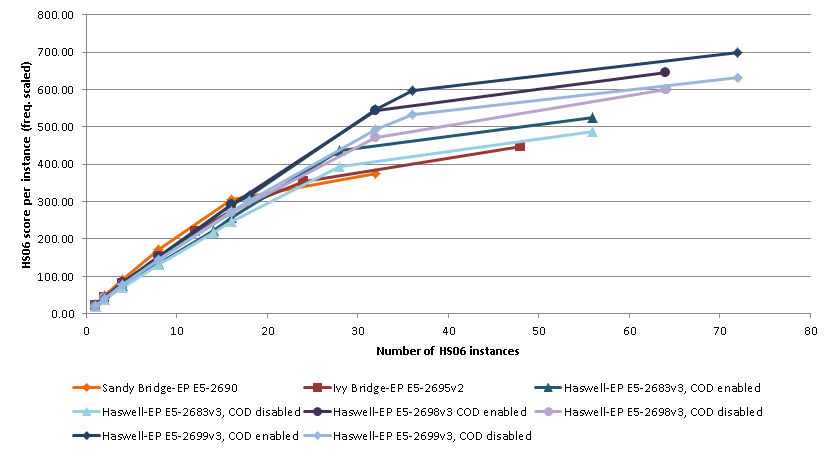
\includegraphics[width=\textwidth]{hs06_absolute}
  \caption{HEP-SPEC06 scalability}
  \label{fig:hs06_absolute}
\end{figure}
\begin{table*}[h]
\centering
\begin{tabular}{@{}cccc@{}}
\toprule
& COD disabled & COD enabled & COD gain \\
\midrule
\textit{Haswell-EP} E5-2683v3 & 486.72 & 524.78 & 7.82\%\\
\textit{Haswell-EP} E5-2698v3 & 600.66 & 644.30 & 7.27\%\\
\textit{Haswell-EP} E5-2699v3 & 631.57 & 700.23 & 10.87\%\\
\bottomrule
\end{tabular}
\caption{HEP-SPEC06 unscaled total scores and performance gains with COD disabled/enabled}
\label{tab:hs06_cod}
\end{table*}

% \begin{table*}[h]
% \centering
% \begin{tabular}{@{}cc@{}}
% \toprule
% & COD disabled\\
% \midrule
% Haswell-EP E5-2683v3 & 486.72\\
% Haswell-EP E5-2698v3 & 600.66\\
% Haswell-EP E5-2699v3 & 631.57\%\\
% \bottomrule
% \end{tabular}
% \caption{HEP-SPEC06 unscaled total scores and performance gains with COD disabled/enabled}
% \label{tab:hs06_cod}
% \end{table*}



\begin{figure}[ht]
\centering
  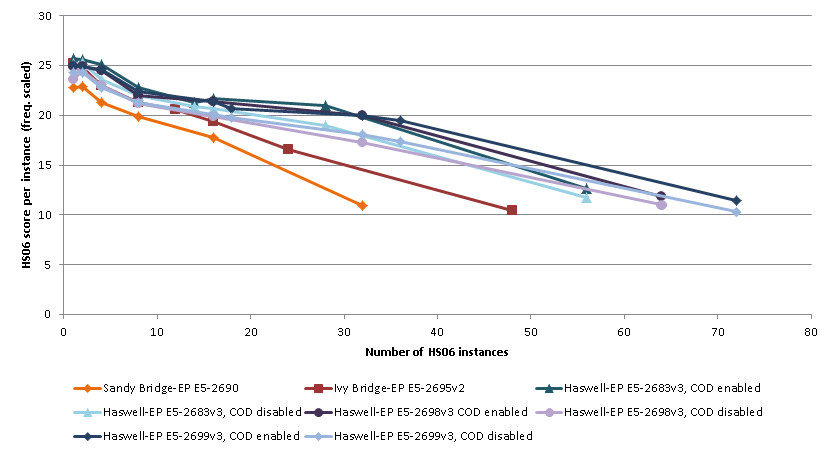
\includegraphics[width=\textwidth]{hs06_per_core}
  \caption{HEP-SPEC06 single core performance scalability}
  \label{fig:hs06_per_core}
\end{figure}




\section{ParFullCMS with Multi-threaded Geant4}

\subsection{Description of the benchmark}
Geant4 (\cite{geant4-1}, \cite{geant4-2}, \cite{geant4-3}) is the major toolkit used in the simulation of the detectors in Large Hadron Collider (LHC). It is used to simulate the passage of particles through matter. It is a principal representative of the workloads run in the Worlwide LHC Computing Grid and constitutes a significant portion of its CPU time. While being multi-threaded, it can exploit multi-threaded parallelism in event processing - once the geometry and the processes are initialized, threads are spawned and events are simulated in parallel. In order to reduce memory footprint, the read-only memory chunks are shared among threads. The version employed in the tests was \verb!geant4-10-01-patch-01!, released on 27.03.2015, built with the default \verb!-O2! optimization flag.

ParFullCMS is a benchmark built on the top of the Geant4 library. It is a stand-alone application implementing a realistic geometry of the CMS detector with full physics simulation, but a simplified setup for data collection, and operating a uniform magnetic-field. It simulates the full geometry of the CMS detector at LHC. To run it, the default physics list QGSP\_BERT was used. The benchmark was built using gcc 4.9.2 with the default compilation flags. The measurement was done by using weak scaling, i.e. keeping the portion of work for each thread constant, while increasing the total number of threads.

\subsection{Description of the experiment}
The ParFullCMS benchmark was used to measure data throughput scalability (i.e. events per second) and power efficiency scalability (i.e. events per joule). In order to collect respective numbers the machines were attached to a power meter while ParFullCMS was launched with with varying number of threads. The application was run in a weak scaling fashion, i.e. while the number of loaded cores was being changed, the workload per core was kept constant making the problem size linear to the number of cores used. At the end of each run the total power consumption over the running time was read out from the device.

\subsection{Results}
Figure \ref{fig:parfullcms_throughput_scalability} shows throughput scalability of the tested platforms. The tested machines provide very similar scalability, with the input of HSW-EP cores being slightly bigger than for their predecessors. When moving to the SMT SNB-EP provides 25\% extra total throughput. IVB-EP and HSW-EP platforms offer very similar gains, being equal to 30\%, 29\%, 32\% and 32\% for E5-2695v2, E5-2683v3, E5-2698v3 and E5-2699v3 respectively. 
\begin{figure}[ht!]
\centering
  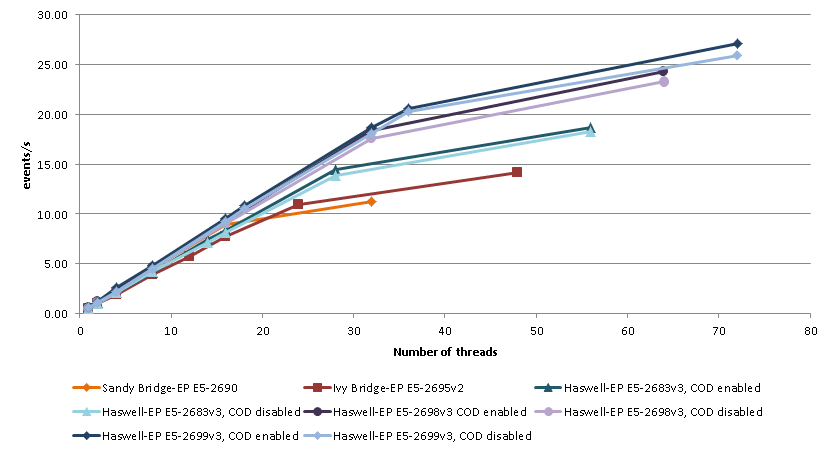
\includegraphics[width=\textwidth]{parfullcms_throughput}
  \caption{ParFullCMS throughput scalability}
  \label{fig:parfullcms_throughput_scalability}
\end{figure}
Figure \ref{fig:parfullcms_power_scalability} shows the power efficiency scalability for the tested platforms, i.e. how many events can be processed per joule with a given number of threads running in parallel. This measurement proves significant in power efficiency in \textit{Haswell-EP} platform. While IVB-EP was able to process 46\% more events per the same amount of energy, \textit{Haswell-EP} is capable of processing up to 102\% more events than IVB-EP and 196\% more than SNB-EP per unit of energy.


\begin{figure}[ht!]
\centering
  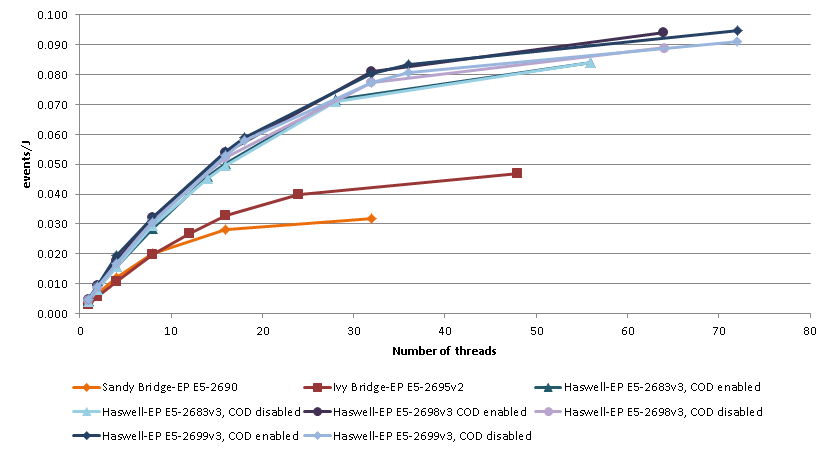
\includegraphics[width=\textwidth]{parfullcms_power}
  \caption{ParFullCMS power efficiency scalability}
  \label{fig:parfullcms_power_scalability}
\end{figure}


\section{VIFit}

\subsection{Description of the benchmark}
VIFit is an evolved version of MLFit \cite{mlfit}. It is a multi-threaded and fully vectorized benchmark, implementing partially the Maximum Likelihood Fit algorithm. It performs a fitting procedure in order to adjust PDF (Probability Density Function) parameters to best reproduce data from the experiment numerical data. To ensure stability of the results VIFit does not perform full minimization - instead the objective function and its gradient is evaluated for a fixed number of points and iterations. It was used to test vectorization performance of the tested plaforms.

VIFit introduces a handful of improvements over its predecessor: runtime is limited to the order of a few seconds, its profile is not dominated by the exp function, the allocated memory can be split into chunks, whose number is defined as a command line parameter, making it NUMA and COD-friendly. Morevore, its performance is intentionally biased by the memory subsystem efficiency.
The benchmark was compiled with gcc 4.9.2 using the following compilation flags: \verb|-funroll-loops|, \verb|-finline-functions| , \verb|-Ofast|, \verb|-ftree-loop-if-convert-stores|, \verb|-fvisibility-inlines-hidden|, \verb|-std=gnu++11|, \verb|-ftree-vectorizer-verbose=1|, \verb|-fopt-info-vec|, \verb|-fipa-pta|. On the top of them we used various vectorization flags in order to produce machine code suitable for different instruction set extenstions: \verb!-mavx2!, \verb!-mavx!, \verb!-msse4.2!, \verb!-fno-tree-vectorize! targeting AVX2, AVX, SSE4.2 and no vectorization, respectively.

The benchmark was run by using as many threads as hardware threads (with SMT) available. The threads were pinned down to the cores.

\subsection{Results}
In the figure \ref{fig:vifit_vector} vectorization speedup obtained with various instruction sets is presented. For each platform non vectorized variant is the baseline. \textit{Haswell-EP} servers provide up to 2x speedup with AVX2 and 1.7x with AVX instruction sets. For every SKU the speedup was higher with COD enabled by 2-2.4\%.
The figure \ref{fig:vifit_speedup} shows speedups of all the tested platforms with respect to SNB-EP, calculated by scaling the run time proportionally to the clock frequency. While the IVB-EP provided 1.5x more performance than SNB-EP (while having 1.5x more cores), the HSW-EP platforms provide 2.91x, 2.99x and 3.14x for E5-2683v3 (1.75x more cores), E5-2698v3 (2x more cores) and E5-2699v3 (2.25x more cores) respectively. This means that, opposed to IVB-EP, we see an additional speedup that is an effect of not only core count increase, but also improvements in the core and uncore architecture.
\begin{figure}[ht!]
\centering
  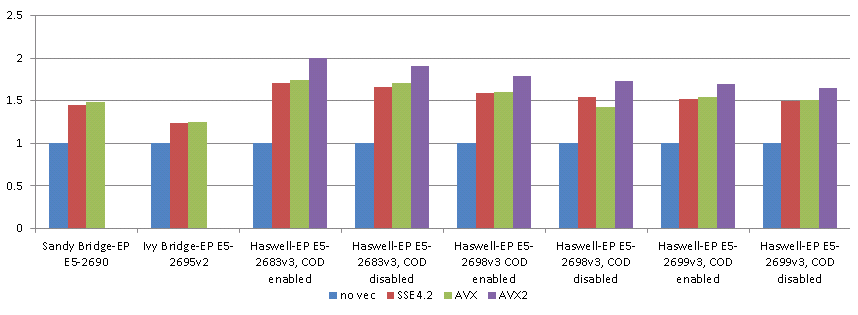
\includegraphics[width=\textwidth]{vifit_vector}
  \caption{Speedups obtained with various target instruction sets. Not vectorized run time was used as a baseline for each platform.}
  \label{fig:vifit_vector}
\end{figure}
\begin{figure}[ht!]
\centering
  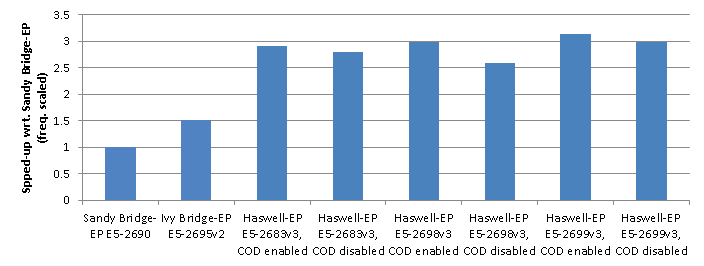
\includegraphics[width=\textwidth]{vifit_speedup}
  \caption{Speedups obtained with respect to Sandy Bridge-EP. Runtimes were scaled proportionally to the clock frequencies.}
  \label{fig:vifit_speedup}
\end{figure}

\section{Conclusions}
The \textit{Haswell-EP} platform provides an across-the-board improvement in performance with respect to the previous generations. The overall performance adventage of 18 cores HSW-EP (E5-2699v3) over 12 cores Ivy Bridge-EP (E5-2695v2) is established at 1.57x speedup for HEP-SPEC06 benchmark, 1.92x better throughput and 2.02x better power efficiency with ParFullCMS and 2.07x for VIFit.
\textit{Haswell-EP} is a platform offering a massive core-count increase with respect to its predecessor, Ivy Bridge-EP. While it maintains the power consumption at a level comparable to IVB-EP, the number of available cores grew by 50\%.

We did not see significant improvement in a single core performance with a legacy single-threaded and not vectorized software. When running HS06 in a weak scaling test we were to achieve higher throuput - proportional to the increase in number of cores.

\textit{Haswell-EP} shows important improvement in the power efficiency. Our experiments with Geant4 and ParFullCMS showed that it can process more than twice more events per unit of energy than IVB-EP.

With \textit{Haswell-EP} the highest speedup obtained in the tests was achieved with VIFit, which is a multi-threaded and highly vectorized workload.
\textit{Haswell-EP} also provides higher vectorization gains than previous dual-socket platforms.

\section*{References}
\bibliographystyle{iopart-num}
\begin{thebibliography}{dupa}
%\bibitem{geant4} Agositnelli S et al. 2003 Geant4 - a simulation toolkit \textit{Nuclear Instruments and Methods in Physics Research Section A: Accelerators, Spectrometers, Detectors and Associated Equipment} \textbf{506} 250-303
\bibitem{geant4-1} Agositnelli S et al. 2003 Geant4 - a simulation toolkit \textit{Nuclear Instruments and Methods in Physics Research Section A: Accelerators, Spectrometers, Detectors} \textbf{506} 250-303
%\bibitem{geant4-2} Allison J et al. 2006 Geant4 developments and applications \textit{IEEE Transactions on Nuclear Science} \textbf{53} 270-278
\bibitem{geant4-3} Dong X, Cooperman G and Apostolakis J 2010 Multithreaded Geant4: Semi-automatic Transformation into Scalable Thread-Parallel \textit{Lecture Notes in Computer Science} \textbf{6272} 287-303
\bibitem{mlfit} Lazzaro A, Jarp S, Leduc J, Nowak A and Valsan L 2012 Report on the parallelization of the MLfit benchmark using OpenMP and MPI \textit{CERN openlab report}
\bibitem{cosmo} Cosmo G 2015 private communication
\end{thebibliography}
\end{document}

